\newpage
\section{Kacper Rothkegel}

\subsection{Photo}
I added a photo of the Windows background (see Figure~\ref{fig:bg}).

\begin{figure}[htbp]
    \centering
    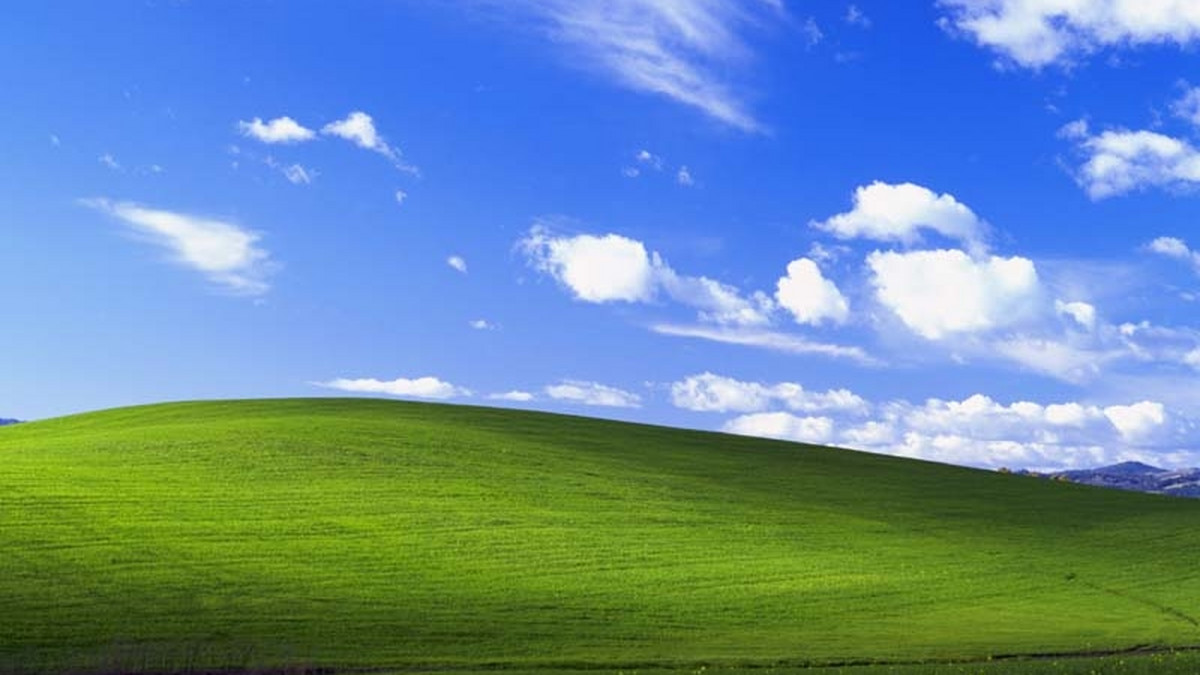
\includegraphics[width=0.3\textwidth]{pictures/tapeta.jpeg}
    \caption{This is a hill}
    \label{fig:bg}
\end{figure}

\subsection{Quote}
\begin{flushright}
The \emph{long, long} road over the moors and up into the forest - who trod it into being \underline{first of all}?\textbf{Man}, a human being, the first that came here.
\end{flushright}

\subsection{Table}
Table~\ref{tab:trigonometric} is below
\begin{table}[h]
\centering
\begin{tabular}{llllll}
+ & 0 & $\frac{\pi}{6}$ & $\frac{\pi}{4}$ & $\frac{\pi}{3}$ & $\frac{\pi}{2}$\\
sin & 0 & $\frac{1}{2}$ & $\frac{\sqrt{2}}{2}$ & $\frac{\sqrt{3}}{2}$ & 1\\
cos & 1 & $\frac{\sqrt{3}}{2}$ & $\frac{\sqrt{2}}{2}$ & $\frac{1}{2}$ & 0 \\
tg & 0 & $\frac{\sqrt{3}}{3}$ & 1 & $\sqrt{3}$ & -
\end{tabular}
\caption{It is trigonometric ratio table}
\label{tab:trigonometric}
\end{table}

\subsection{Lists}
This is an unordered list
\begin{itemize}
  \item yes
  \item no
\end{itemize}

This in an ordered list
\begin{enumerate}
  \item one
  \item two
\end{enumerate}

\subsection{Math equations}
Here is quite an interesting equation
$ a^2 = b^2 + c^2 -2bccos(\alpha)  $

And here it is even more interesting
\[b^2m + c^2n = a(d^2 + mn)\]

